% -*- Mode: noweb; noweb-default-code-mode: R-mode; -*-
%\SweaveUTF8
\documentclass[11pt]{article}\usepackage[]{graphicx}\usepackage[]{color}
%% maxwidth is the original width if it is less than linewidth
%% otherwise use linewidth (to make sure the graphics do not exceed the margin)
\makeatletter
\def\maxwidth{ %
  \ifdim\Gin@nat@width>\linewidth
    \linewidth
  \else
    \Gin@nat@width
  \fi
}
\makeatother

\definecolor{fgcolor}{rgb}{0.345, 0.345, 0.345}
\newcommand{\hlnum}[1]{\textcolor[rgb]{0.686,0.059,0.569}{#1}}%
\newcommand{\hlstr}[1]{\textcolor[rgb]{0.192,0.494,0.8}{#1}}%
\newcommand{\hlcom}[1]{\textcolor[rgb]{0.678,0.584,0.686}{\textit{#1}}}%
\newcommand{\hlopt}[1]{\textcolor[rgb]{0,0,0}{#1}}%
\newcommand{\hlstd}[1]{\textcolor[rgb]{0.345,0.345,0.345}{#1}}%
\newcommand{\hlkwa}[1]{\textcolor[rgb]{0.161,0.373,0.58}{\textbf{#1}}}%
\newcommand{\hlkwb}[1]{\textcolor[rgb]{0.69,0.353,0.396}{#1}}%
\newcommand{\hlkwc}[1]{\textcolor[rgb]{0.333,0.667,0.333}{#1}}%
\newcommand{\hlkwd}[1]{\textcolor[rgb]{0.737,0.353,0.396}{\textbf{#1}}}%
\let\hlipl\hlkwb

\usepackage{framed}
\makeatletter
\newenvironment{kframe}{%
 \def\at@end@of@kframe{}%
 \ifinner\ifhmode%
  \def\at@end@of@kframe{\end{minipage}}%
  \begin{minipage}{\columnwidth}%
 \fi\fi%
 \def\FrameCommand##1{\hskip\@totalleftmargin \hskip-\fboxsep
 \colorbox{shadecolor}{##1}\hskip-\fboxsep
     % There is no \\@totalrightmargin, so:
     \hskip-\linewidth \hskip-\@totalleftmargin \hskip\columnwidth}%
 \MakeFramed {\advance\hsize-\width
   \@totalleftmargin\z@ \linewidth\hsize
   \@setminipage}}%
 {\par\unskip\endMakeFramed%
 \at@end@of@kframe}
\makeatother

\definecolor{shadecolor}{rgb}{.97, .97, .97}
\definecolor{messagecolor}{rgb}{0, 0, 0}
\definecolor{warningcolor}{rgb}{1, 0, 1}
\definecolor{errorcolor}{rgb}{1, 0, 0}
\newenvironment{knitrout}{}{} % an empty environment to be redefined in TeX

\usepackage{alltt}
\usepackage{graphicx}
%% \usepackage{Sweave}
\usepackage[utf8]{inputenc}
%% \usepackage{germanU}
%%- \usepackage[noae]{Sweave}
\usepackage[a4paper, text={14.5cm,22cm}]{geometry}
\usepackage{color} %uncomment BF
\usepackage{booktabs} % nice tables with \toprule \middlerule \bottomrule
\usepackage{amsmath} % for align
% \usepackage{wasysym} % for promille sign
% \usepackage{amssymb}
% \usepackage[textfont=it,font=small,labelfont=it]{caption}
\interfootnotelinepenalty=10000 % prevent LaTex from two-sided footnotes
\usepackage{pldescr}
%% \VignetteEngine{knitr::knitr}
\def\wh#1{\widehat{#1}}

\addtolength{\textwidth}{2.5cm}%%--- 15.0 + 2.5 = 17.5
\addtolength{\oddsidemargin}{-1.04cm}

%% ================================================================
\IfFileExists{upquote.sty}{\usepackage{upquote}}{}
\begin{document}
%% \SweaveOpts{concordance=TRUE,width=9,height=6, echo=false}
\setkeys{Gin}{width=1\textwidth}
\baselineskip 15pt
\parskip 10pt

\title{\vspace*{-10mm}
'plgraphics': A user-oriented collection of graphical R-functions based on
 the 'pl' concept}
\author{Werner A. Stahel, ETH Zurich}
\maketitle

\begin{abstract}\noindent
The package, \T{plgraphics}, collects enhanced versions of basic plotting
functions. It is based on a paradigm between the basic R graphics elements
and the more computer science oriented ggplot concepts.
The intention is to furnish user-oriented functions that allow efficient
production of useful graphics.
\end{abstract}



\section{Introduction}

The plotting functionality is the historical origin of the R package.
It has been introduced half a century ago and has grown for a while.
For the sake of upward compatibility, it has been essentially unchanged for
several decades. 

New graphical concepts, adjusted to the development of graphical devices
and computer science ideas have been implemented in new packages, 
notably \T{ggplot} ...

The intention of the package \T{plgraphics} is to implement some functions
that provide efficient production of simple to rather sophisticated plots,
but are still based on the core R functionality.
They have been developed over a long time with a focus on allowing 
for readily interpretable graphical diagnostics for regression model
development. 

The general idea is that it should be easy to produce standard plots 
by calling \T{plot(x,y)} or \T{plot(y$\sim$x, data=dd)}, 
as well as enhancing the plot by adding an argument \T{smooth=T} 
to ask for a smoother or specifying 
a column in the dataset that drives the color or yields labels to mark the
points to be shown. 
The plots should remain useful if there are outliers of one of the two
variables is a grouping factor instead of a quantitative variable.

Asking that a basic function provides many variations under the control of
the user means that a large list of arguments must be available.
Some of these variations depend on the taste of the user. 
They can be specified in a kind of ``style'' list, analogous to 
\T{options} and \T{par}, which is called \T{userOptions}.

The package also provides enhanced low level graphical functions
like \T{plpoints}, which extends the functionality of \T{points}.
This leads to a very short basic scatterplot function \T{plyx} that can
easily be modified by the user.

This document presents the main features of the package \T{plgraphics}
and explains the concepts behind them. 

The package \emph{will be} available from \T{R-forge}, e.g. by calling\\
\T{install.packages("plgraphics", repos="http://r-forge.r-project.org")}.\\

\section{Scatterplots}

\subsection{The basic scatterplot}
A basic scatterplot is generated by calling \T{plyx}
(plot y on x).

\begin{knitrout}
\definecolor{shadecolor}{rgb}{0.969, 0.969, 0.969}\color{fgcolor}\begin{kframe}
\begin{alltt}
\hlkwd{plyx}\hlstd{(Sepal.Width}\hlopt{~}\hlstd{Sepal.Length,} \hlkwc{data}\hlstd{=iris,} \hlkwc{smooth}\hlstd{=}\hlnum{FALSE}\hlstd{)}
\end{alltt}
\end{kframe}
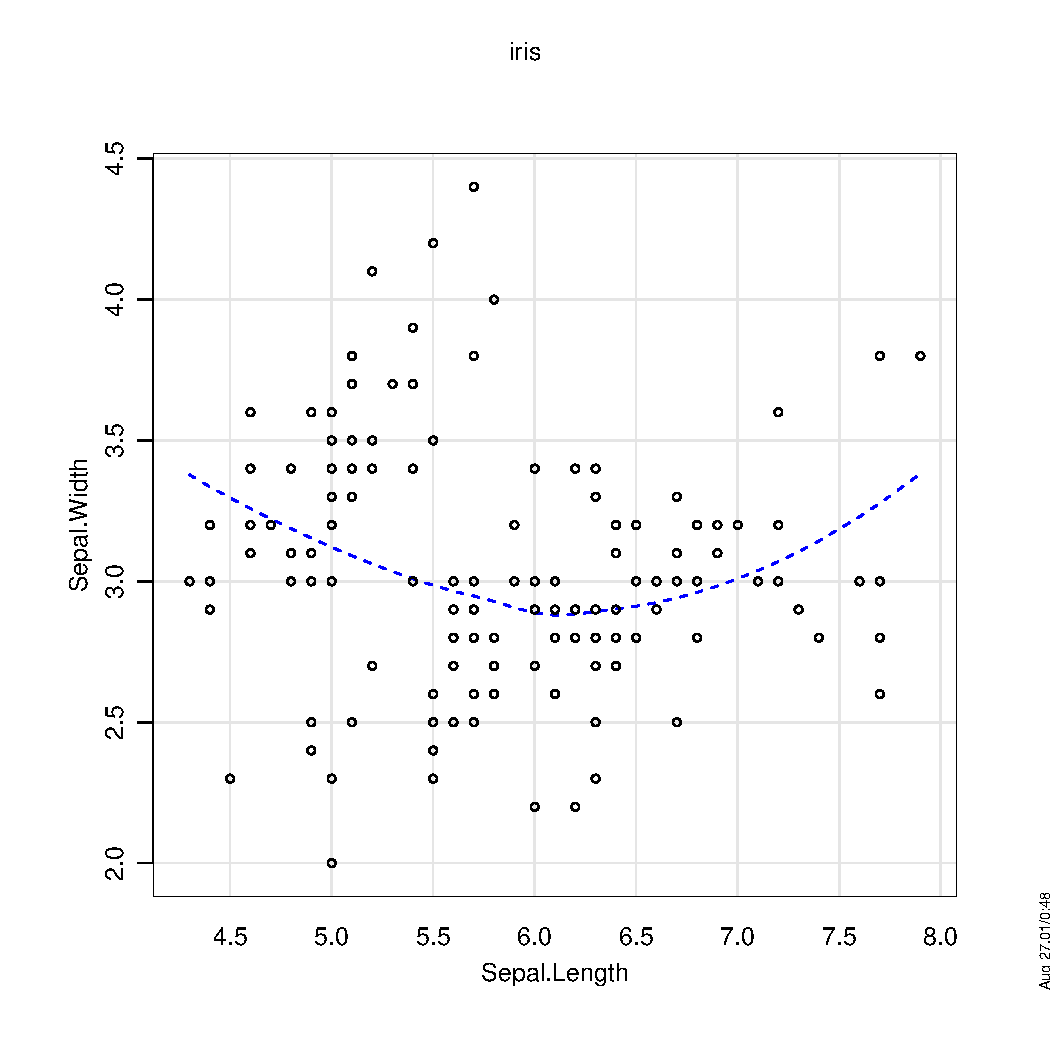
\includegraphics[width=\maxwidth]{figure/plyx-1} 

\end{knitrout}
Clearly, this stongly resembles the result of simply calling \T{plot}, 
except for the thin gridlines and some documentation added by default: 
The name of the dataset is shown as a (sub-) title, and there is a small
text in the lower right corner that shows the date.
%% and a project label that has been set by typing 
%% \T{options(project="pl documentation")}.
Without \T{smooth=FALSE}, a smooth line is added, see below.

More arguments allow to specify many aspects of the plot.
\begin{knitrout}
\definecolor{shadecolor}{rgb}{0.969, 0.969, 0.969}\color{fgcolor}\begin{kframe}
\begin{alltt}
\hlkwd{plyx}\hlstd{(Sepal.Width}\hlopt{~}\hlstd{Sepal.Length,} \hlkwc{data}\hlstd{=iris,}
     \hlkwc{psize}\hlstd{=Petal.Length}\hlopt{^}\hlnum{2}\hlstd{,} \hlkwc{pcol}\hlstd{=Species,} \hlkwc{pch}\hlstd{=Species,} \hlkwc{cex}\hlstd{=}\hlnum{1.5}\hlstd{)}
\end{alltt}
\end{kframe}
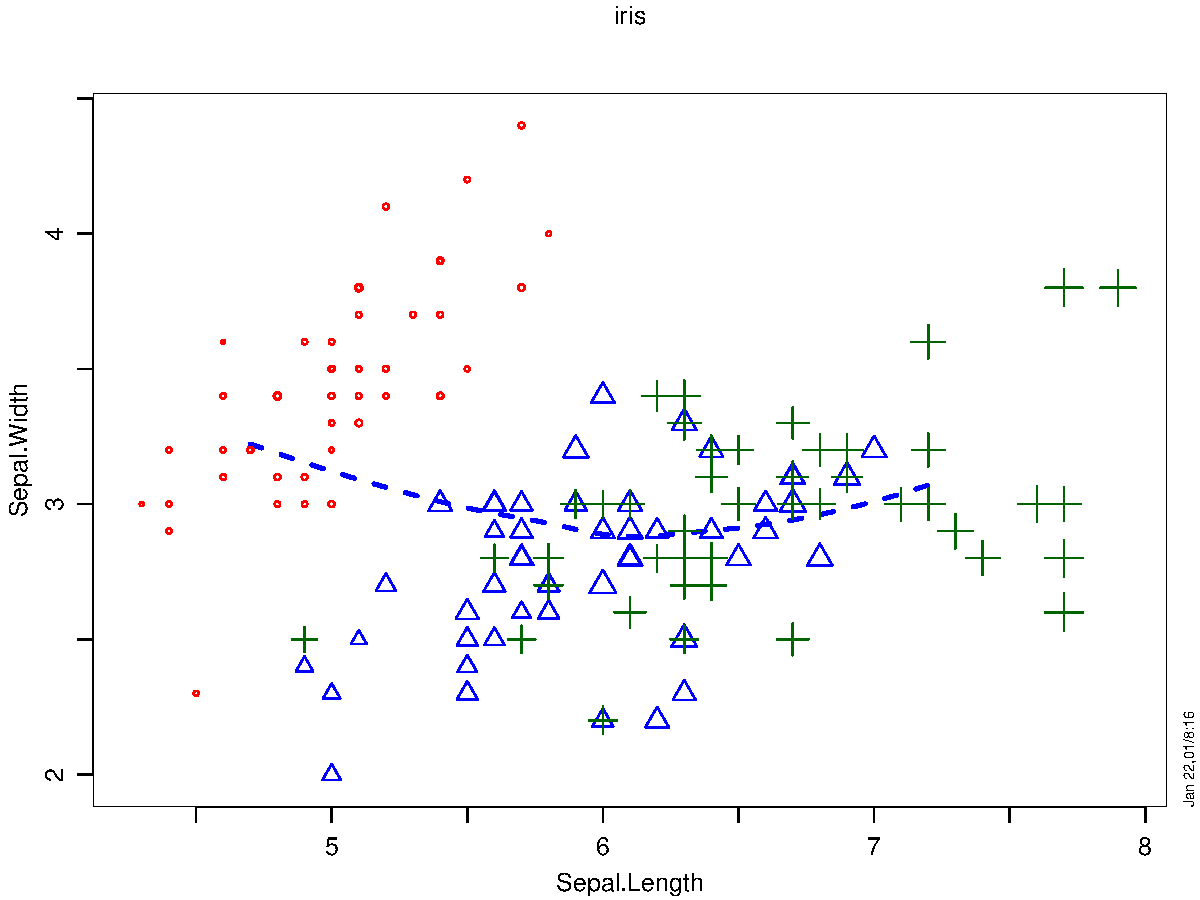
\includegraphics[width=\maxwidth]{figure/plyx_pchar-1} 

\end{knitrout}
The argument \T{psize}) sets the size of the plotting symbols
such that their area is proportional to it.
The median size is determined by \T{cex}.
By default, this value adjusts to the number of observations.

See ... for details.

\Tit{Smooth.}
A smooth line fitting the data in the plot is requested by typing
\T{smooth=TRUE}. The line type, width and color are modified by
respective arguments.

Smooths can also be fitted groupwise by specifying \T{smooth.group}.

\begin{knitrout}
\definecolor{shadecolor}{rgb}{0.969, 0.969, 0.969}\color{fgcolor}\begin{kframe}
\begin{alltt}
\hlkwd{plmfg}\hlstd{(}\hlnum{1}\hlstd{,}\hlnum{2}\hlstd{)}
\hlkwd{plyx}\hlstd{(Sepal.Width}\hlopt{~}\hlstd{Sepal.Length,} \hlkwc{data}\hlstd{=iris,} \hlkwc{smooth}\hlstd{=}\hlnum{TRUE}\hlstd{,} \hlkwc{smoothlines.col}\hlstd{=}\hlstr{"red"}\hlstd{)}

\hlkwd{plyx}\hlstd{(Sepal.Width}\hlopt{~}\hlstd{Sepal.Length,} \hlkwc{data}\hlstd{=iris,} \hlkwc{smooth}\hlstd{=}\hlnum{TRUE}\hlstd{,} \hlkwc{smooth.group}\hlstd{=Species,}
     \hlkwc{pcol}\hlstd{=Species)}
\end{alltt}
\end{kframe}
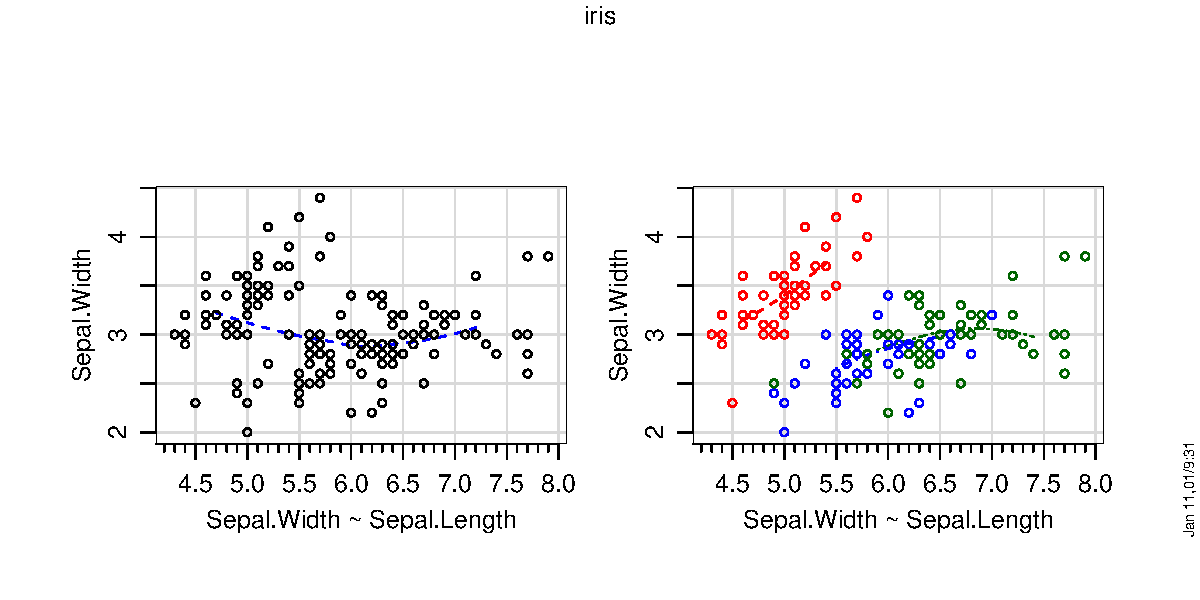
\includegraphics[width=\maxwidth]{figure/plyx_smooth-1} 

\end{knitrout}
Setting \T{pcol=Species} allowed the color of plotting symbols and smooth
lines to be the same.

If the argument \T{group} is specified, separate plots will be generated
for the different groups, thereby maintaining the plot ranges.

\begin{knitrout}
\definecolor{shadecolor}{rgb}{0.969, 0.969, 0.969}\color{fgcolor}\begin{kframe}
\begin{alltt}
\hlkwd{plmfg}\hlstd{(}\hlnum{2}\hlstd{,}\hlnum{2}\hlstd{)}

\hlkwd{plyx}\hlstd{(Sepal.Width}\hlopt{~}\hlstd{Sepal.Length,} \hlkwc{data}\hlstd{=iris,} \hlkwc{smooth}\hlstd{=}\hlnum{TRUE}\hlstd{,} \hlkwc{group}\hlstd{=Species)}
\end{alltt}
\end{kframe}
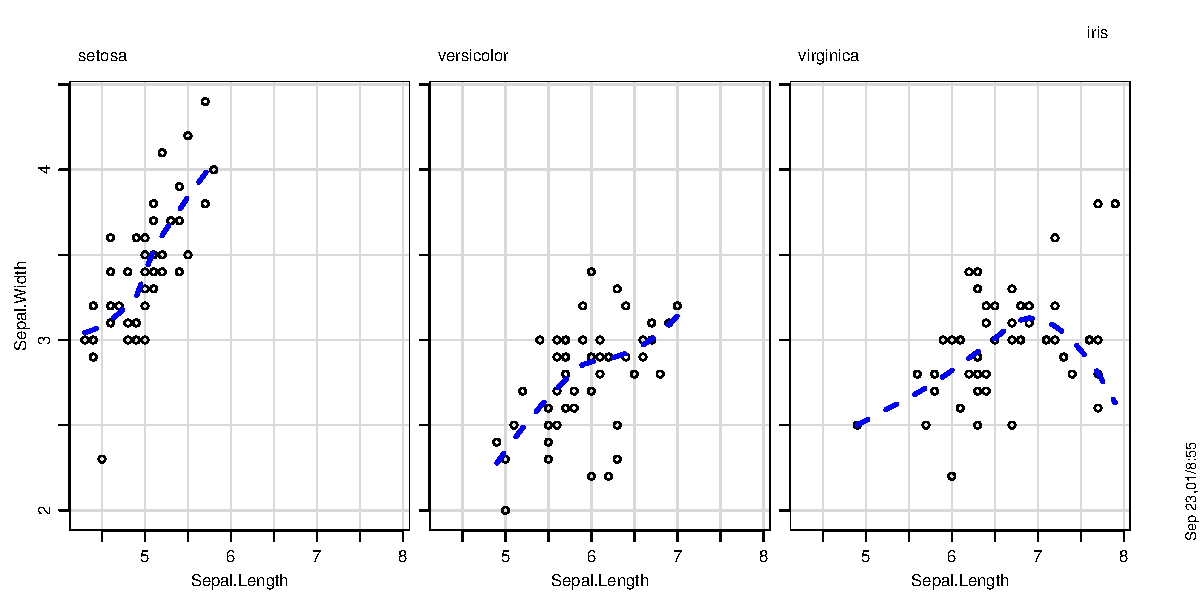
\includegraphics[width=\maxwidth]{figure/plyx_group-1} 

\end{knitrout}
%% !!! farbe stimmt nicht -- und lty wohl auch nicht.

\Tit{Inner range of plots.}
When there are outliers in the data, plots are dominated by their effect of
determining the plotting range. This means that the user who would like to
see more detail about the ``regular'' observations needs to gnerate a new
plot, specifying the limits of the plotting range by \T{xlim} and \T{ylim}.

In order to avoid the urge for two versions of the plot, an ``inner
plotting range'' is determined, based on robust measures of 
location and scale. Outside this range, there is a plotting margin where
coordinates are transformed with a highly nonlinear function in order to
accomodate all outliers. 
In these margins, the order of coordinates is still maintained, thus
allowing to see which points are further out than others, but quantitative
information is distorted by the transformation.
The figure shows data from the blasting example with an added outlier,
plotted without and with inner plotting limits.

\begin{knitrout}
\definecolor{shadecolor}{rgb}{0.969, 0.969, 0.969}\color{fgcolor}\begin{kframe}
\begin{alltt}
\hlkwd{data}\hlstd{(d.blast)}
\hlstd{dd} \hlkwb{<-} \hlstd{d.blast}
\hlstd{dd}\hlopt{$}\hlstd{distance[}\hlnum{2}\hlstd{]} \hlkwb{<-} \hlnum{200}
\hlkwd{plmfg}\hlstd{(}\hlnum{1}\hlstd{,}\hlnum{3}\hlstd{)}
\hlkwd{plyx}\hlstd{( tremor}\hlopt{~}\hlstd{distance,} \hlkwc{data}\hlstd{=dd,} \hlkwc{innerrange}\hlstd{=}\hlnum{FALSE}\hlstd{)}
\hlkwd{plyx}\hlstd{( tremor}\hlopt{~}\hlstd{distance,} \hlkwc{data}\hlstd{=dd)}
\hlkwd{plyx}\hlstd{( tremor}\hlopt{~}\hlstd{distance,} \hlkwc{data}\hlstd{=dd,} \hlkwc{innerrange.factor}\hlstd{=}\hlnum{5}\hlstd{)}
\end{alltt}
\end{kframe}
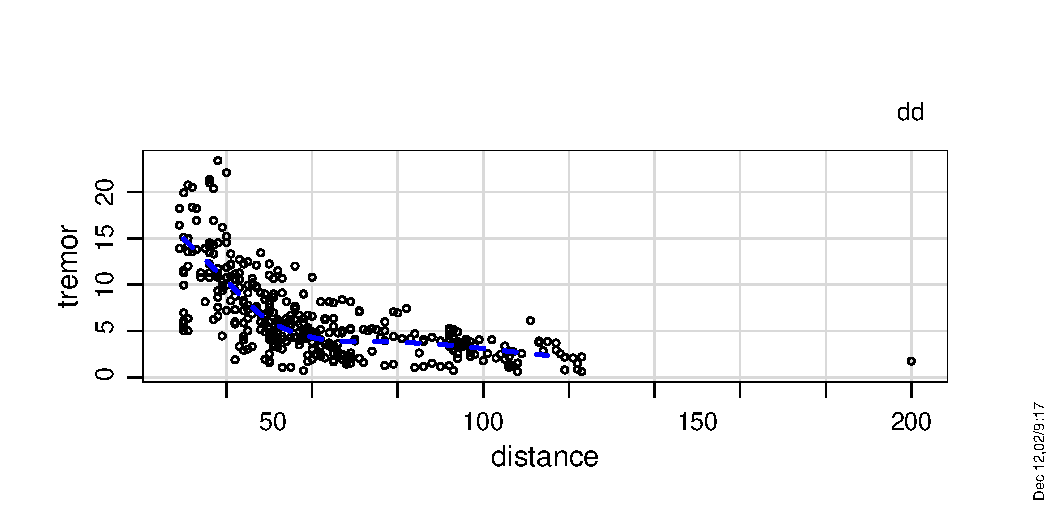
\includegraphics[width=\maxwidth]{figure/innerrange-1} 

\end{knitrout}

If \T{innerrange=TRUE}, which is the default, the \T{plgraphics} functions
will determine an ``inner plotting range'' based on 
the 20\% trimmed mean and a 20\% trimmed scale by default.


%% innerrange
\Detail{The function \T{robrange}, which is called by \T{plinnerrange},
  determines the $\alpha$-trimmed mean with $\alpha=0.2$ as the location 
  and the (one-sided) trimmed mean of the deviations from it. 
  It adjusts this latter mean to obtain an approximately consistent
  estimate of the standard deviation for normal observations to obtain the 
  scale estimate. It then calculates the location plus-minus 
  \T{innerrangeFactor} times the scale to get a potential inner range.
  The final inner plotting range will be the intersection of this and the
  ordianry range of the values.
}
%% ------------------------------

\subsection{Multiple y and x}
Two or more variables may be given to be plotted on the vertical axis,
in the sense of \T{matplot} of R.
Often, these are parallel time series, and it is convenient to ask for 
lines connecting the points, either \T{type="l"} or \T{type="b"}.
\T{plyx} will choose different scales for the different variables unless
\T{rescale=FALSE}.

\begin{knitrout}
\definecolor{shadecolor}{rgb}{0.969, 0.969, 0.969}\color{fgcolor}\begin{kframe}
\begin{alltt}
\hlkwd{plyx}\hlstd{(}\hlnum{1}\hlopt{:}\hlnum{40}\hlstd{, EuStockMarkets[}\hlnum{1}\hlopt{:}\hlnum{40}\hlstd{,],} \hlkwc{type}\hlstd{=}\hlstr{"b"}\hlstd{)}
\end{alltt}
\end{kframe}
\includegraphics[width=\maxwidth]{figure/plyx_multipley-1} 

\end{knitrout}

If multiple x variables are given, a separate plot is drawn for each of them.

\subsection{Marking extreme points}
%% markextremes
The default value of \T{markextremes} is 0 for \T{plyx}.
If the argument is \T{NA}, it depends on the number of 
observations: It is $1/(2\sqrt{n})$. 

\Tit{Factors, \T{mboxes}}

\Tit{Censored data}

\Tit{Raw or transformed variables?}
max(x1,x2)

\begin{knitrout}
\definecolor{shadecolor}{rgb}{0.969, 0.969, 0.969}\color{fgcolor}\begin{kframe}
\begin{alltt}
\hlstd{t.plopt} \hlkwb{<-} \hlkwd{ploptions}\hlstd{(}\hlkwc{basic.col}\hlstd{=}\hlstr{"blue"}\hlstd{)}
\hlkwd{plyx}\hlstd{(Sepal.Width}\hlopt{~}\hlstd{Sepal.Length,} \hlkwc{data}\hlstd{=iris,} \hlkwc{ploptions}\hlstd{=t.plopt)}
\end{alltt}
\end{kframe}
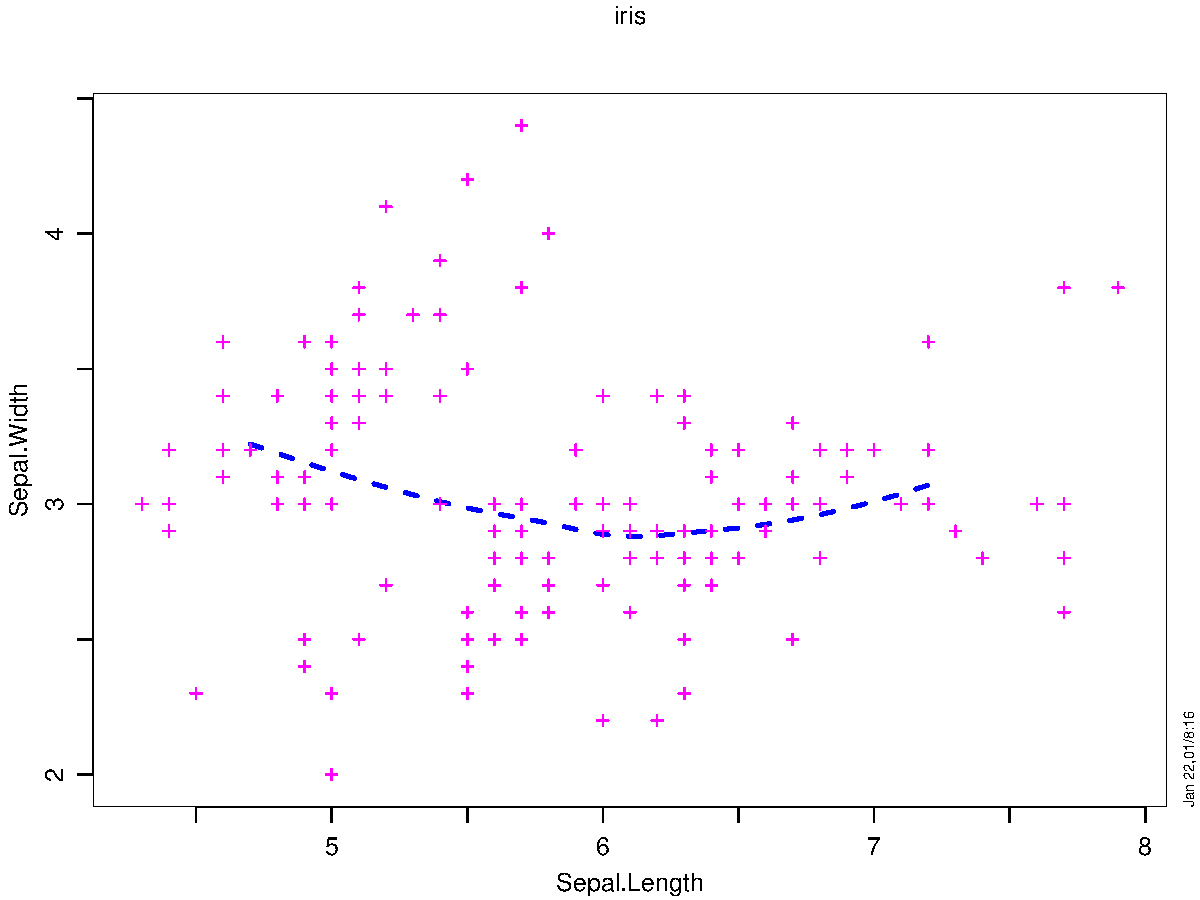
\includegraphics[width=\maxwidth]{figure/ploptions-1} 

\end{knitrout}


\section{Scatterplot matrix}

\Tit{Multiple x}

\Tit{Groups}

\Tit{Same scales}

\T{plmatrix}

\section{Regression diagnostic plots}

diagnostics should be specific 
scale diagnostic should work even when bias is signalled

\T{plot.regr}

\Tit{Residuals against fit}

\Tit{Absolute residuals against fit}
residuals from smooth
censored: no intervals

\Tit{QQ-plot}
only for Gaussian

markextremes

\Tit{plresx}
This function plots the residuals against the input variables,
either in raw or in transformed form.

The raw input variables are those appearing in the formula, as delivered by
\T{all.vars(formula)}.

The transformed input variables are those appearing in the terms of the
formula, as delivered by \T{rownames(attr(terms(formula[1:2]), "factors"))}.

fitcomp: use model.frame -> model.matrix -> lm.fit

  
  


plrex2x

%% ==============================================================
\section{Options}

\Tit{ploptions}
The graphical elements, like plotting character, color, line types, etc. 
to be used in pl graphics are specified in the pl options. 
They are analogous to the ordinary options, with two differences:
\Itm
The pl options are stored in a list \T{.ploptions} which is not erased when
leaving the R session. It can therefore be stored with the global
environment. 
\Itm
There is a list \T{ploptionsDefault} in the package. It collects the
packages default settings and is used as a backup if some components should
not be contained in \T{.ploptions}.

The function \T{ploptions} is used to set and get pl options, in the same
way that \T{options} sets and gets the basic R options.

The basic concept behind the pl option list is that all pl functions use it
as a resource to find the graphical elements.

Remark:
This concept is a version of a more general idea, saying that 
the default values of any ``high level'' R function should have an
associated list of default arguments, which is not contained in the
function definition, but stored separately. 
This allows the user to specify his own style by changing these defaults
and storing them in a kind of style file to be loaded at the start of each
session. 
Here, there is only one list because the pl functions need the same
graphical elements.

Thus, a graphical element like a plotting character is generally searched 
in
\begin{enumerate}
\item 
  the argument list of the calling function
\item
  the \T{ploptions} argument of the calling function
\item
  the \T{.ploptions} list
\item
  the list \T{ploptionsDefault} in the package \T{plgraphics}
\end{enumerate}

%% ---------------------------------
\Tit{Plotting data}

pdata
attributes of points, grouping

plotting elements for grouping

attributes of variables
label
axis
colors  lty, lwd?)
to be used if variable is plotted vertically (only if multiple vars?)

very often NULL, adaptation to data

\Tit{.parguments}

Some graphical elements will depend on the number of observations
  default: cex
  
title: cex, cexmin
  

\section{Low level graphics and auxiliary functions}

plframe, 

plpoints, 
  plab; pch for is.na(plab)  or  plab==""
  cex: plappearance\$cex * plappearance\$default\$cex
  (priorities for) plotting character
  censored

plsmooth, plsmlines, 

plreflines

pltitle
adaptation of cex

pllimits, plcoord



\section{Details}

\subsection{plargs, ploptions, default values} 
(if needed, see above)

\Tit{Default values}
\T{i.def}
\T{i.getploption} and \T{i.getplopt}

Some arguments to low level pl functions need to be set by changing
the \T{ploptions} argument.
Example:

residuals in pargs are data.frame

variable colors, ... stored in pdata
generated in pl.control avoiding elements already in use 

\subsection{Components of plptions}

\Tit{innerrange}
Usually, \T{innerrange} is a logical, indicating if inner ranges
should be determined
\T{innerrange.limits} is a vector of length 2 giving the range to be
applied. 

?? Both can also be a named list of such objects, where the names reflect the 
variables.

set innerrange.limits by calling genvarattributes



\subsection{Point labelling and plotting character}
Priorities:
\begin{enumerate}
\item 
  If they are specified by the respective argument to high level \T{pl} 
  function (and evaluated by \T{pl.control}), this has priority
  (excemption, see 2.).
\item
  In the case of multiple $y$s, colors are determined primarily by 
  the argument \T{ycol} of the high level \T{pl} function, 
  scondarily by the \T{col} attribute of the variables. 
  Thirdly, the \T{variables} component of \T{plappearance} is used,
  avoiding colors that are already specified for some variables by the
  foregoing steps. 
  [See \T{i.getPlattributes}, called by \T{genvarattributes} in 
  \T{pl.control}.]\\
  If \T{pch} is not determined otherwise (argument, see 1., or group,
  see 3.) it is set in the same way.\\
  For plots of type \T{l} or \T{b}, the line type \T{lty} is determined 
  in the same way as the color.
\item
  If there is grouping and only a single $y$, the group determines \T{pch}
  and its color by the \T{group} component of \T{plappearance} unless set
  by 1. above.
\item
  In other cases, the \T{default} component of \T{plappearance} is used.
\end{enumerate}

\subsection{Groups}

\Tit{Color}
If color (\T{pcol}) is a factor, it will be converted into 
\T{ploptions("group.col")[as.numeric(pcol)]}.
In order to give color by color names, make sure that \T{pcol} is
a character variable.

\subsection{Standardized residuals}

\[
R^*_i=R_i\left/\left(\wh\sigma \sqrt{w_i} \sqrt{1-H_{ii}}\right)\right.
\]

Standardization ratio: 
$\T{stratio}_i=R^*_i/R_i$

\T{i.stres} calculates leverages, standardized residuals, and \T{strratio}
according to this formula.
For binary and Poisson models, ...

Cook's distance:
\[
  d_i\sups C=\frac{R_i^2\,H_{ii}}{p\wh\sigma^2\,(1-H_{ii})^2}
  =(1/p)\,R_i^{*2}\,H_{ii}/(1-H_{ii})
  \;,
\]
It is constant, $=d$, on the curve
\[
  R_i^{*2} = d\,p\,(1-H_{ii})/H_{ii}
\]
A rule suggests $d=4/(n-p)$ as a warning level.
Curves are drawn for $d=\T{cookdistlines}^2/(n-p)$.

%% =================================================================
{\small
\Tit{This is the end} of the story for the time being. I hope that you will
get into using \T{regr} and have good success with your data analyses.
Feedback is highly appreciated.

Werner Stahel, \T{stahel at stat.math.ethz.ch}
}
\end{document}

%%% Local Variables: 
%%% mode: latex
%%% TeX-master: t
%%% End: 
